\chapter{NCMC Switching}

\section{Introduction}
%
If new atoms are introduced into a condensed-phase simulation, it is highly likely that they will be placed unfavorably close to other atoms.
%
Additionally, if a ligand is transforming to another ligand, valence and nonbonded terms may also need to transform, as demonstrated in Figure~\ref{fig:benz_chlorobenz}
%
In order to mitigate these very serious issues, we turn to Nonequilibrium Candidate Monte Carlo (NCMC)~\cite{Nilmeier2011}. 
%
NCMC is a technique that allows us to gradually interpolate the system from one set of control parameters to another.
%
In this particular case, atoms are introduced after dimension matching as non-interacting dummies, and core atoms are left with their original parameters.
%
Then, the algorithm alternates between incrementing the control parameters and taking one step of Langevin dynamics (or other MCMC algorithm that either maintains the invariant distribution, or accounts for deviations by including an importance weight)
%
This allows new atoms to be introduced smoothly, and allows core atoms to be smoothly interpolated from one set of parameters to another.
%
\begin{figure}[H]
    \centering
    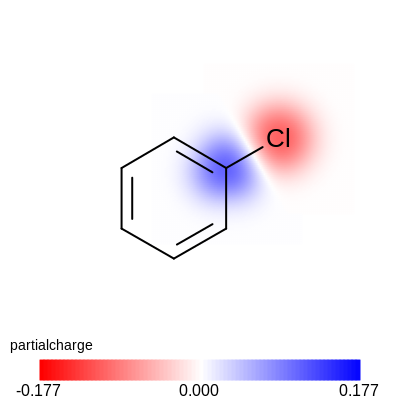
\includegraphics[width=0.5\textwidth]{partialcharge-pm.png}
    \caption{Chlorobenzene, with atoms colored by charge. If the ring is mapped to benzene (where all partial charges are equal), the abrupt change is very unfavorable.}
    \label{fig:benz_chlorobenz}
\end{figure}
%
\section{Description of Algorithm}
%
In broad terms, the algorithm performs the following steps:
\begin{itemize}
    \item Given system A, system B, and an atom map between them, generate hybrid system H with control parameters $\lambda \in [0,1]$
    \item Perform annealing or nonequilibrium switching, changing control parameters from 0 to 1 gradually and accumulating the change in energy
    \item Transfer the positions to system B
\end{itemize}
%
\subsection{Construction of Hybrid System}
%
The first step is to construct a system that is the hybrid of the two endpoints.
%
The object of constructing this system is to be able to smoothly interpolate from the first endpoint to the second.
%
To that end, I build the system with modified energy terms: all of the terms are controllable through global parameters collectively known as $\lambda$.
%
When $\lambda=0$, the hybrid system behaves like the initial endpoint.
%
When $\lambda=1$, the hybrid system behaves like the final endpoint.
%
The construction of such a system, as well as the path that one takes through the space of control parameters, are important factors in the performance of the overall algorithm.
%
Here, I will describe in greater detail the way that each type of energy term for a classical forcefield is handled.
%
\subsubsection{Bond force}
%
In the AMBER forcefields~\cite{Ponder2003}, bond forces are represented by a harmonic term:
%
\begin{equation} \label{eq:bondforce}
    U(r) = \frac{K_r}{2}(r - r_0)^2
\end{equation}
\noindent where the $K$ is a force constant and the $r_0$ is the equilibrium bond length. 
%
For bonds present in both endpoint systems in the region of the system that is being modified, I use a slightly modified potential:
\begin{eqnarray} \label{harmonic_alchemical}
    r_0 (\lambda_{bonds}) = (1 - \lambda_\mathrm{bonds}) r_{0_A} + \lambda_\mathrm{bonds} r_{0_B} \\
    K_r (\lambda_{bonds}) = (1 - \lambda_\mathrm{bonds}) K_{r,A} + \lambda_\mathrm{bonds} K_{r,B} \\
    U(r; \lambda_{bonds}) = \frac{K_{r} (\lambda_\mathrm{bonds})} {2} \left[ r - r_0(\lambda_\mathrm{bonds}) \right]^2
\end{eqnarray}
%
\noindent In this way, the hybrid system's bond energy linearly depends on the control parameter $\lambda_{bonds}$ between the endpoints.
%
We are also free to change the bond parameters nonlinearly with the master $\lambda$ control parameter's schedule.
%
For bonds that are not in the modified region, a standard harmonic term is used. 
%
Likewise, for bonds between atoms that only exist in one endpoint or the other, a standard harmonic term is used to prevent them from departing the region where they belong.
%
A tricky issue arises when two atoms are present in both systems, but have a bond only in one.
%
This arises in the case of transforming a non-ring into a ring.
%
In this case, for the system without the ring, the bond force constant is set to 0. 
%
However, it should be noted that these proposals are likely not desirable, and should be remedied by reducing the number of atoms in the map.
%
Finally, it is important to mention that when a constrained bond is encountered, its constraint length is not changed.
%
This is to avoid the need to compute a Jacobian for this deterministic transformation, although it would in principle be possible.
%
I have found that this issue can generally be avoided entirely by simply not mapping hydrogen atoms.
%
\subsubsection{Angle force}
%
Also included in AMBER force fields (as well as others) are angle terms between 3 atoms.
%
These force terms are also harmonic, with the form:
%
\begin{equation} \label{eq:angleforce}
    U(r) = \frac{K_{\theta}}{2}(\theta - \theta_0)^2
\end{equation}
%
I treat these similarly to the bonds in \ref{harmonic_alchemical}:
%
\begin{eqnarray} \label{harmonic_alchemical_angles}
    \theta_0 (\lambda_{angles}) = (1 - \lambda_\mathrm{angles}) \theta_{0_A} + \lambda_\mathrm{angles} \theta_{0_B} \\
    K_\theta (\lambda_{angles}) = (1 - \lambda_\mathrm{angles}) K_{\theta,A} + \lambda_\mathrm{angles} K_{\theta,B} \\
    U(\theta; \lambda_{angles}) = \frac{K_\theta (\lambda_{angles})} {2}\left[\theta - \theta_0(\lambda_{angles})\right]^2
\end{eqnarray}
%
As with the bonds, I do not use the modified potential for angles that are not in the region being modified, nor do I use them for triplets of atoms that are only present in one endpoint.
%
The ring closure issue is also present with the angles, and is handled similarly.
%
\subsubsection{Dihedral force}
%
Dihedral angles also have potential terms, of the form:
%
\begin{equation}
    U(\phi) = \sum_{l=1}^L \frac{K_{\phi,l}}{2} \cos(n_l \phi - \gamma_l)
\end{equation}
%
\noindent where $\phi$ is the dihedral angle, and for Fourier component $l \in \{1, \ldots, L\}$, $n_l$ is the periodicity, $\gamma_l$ is the phase, and $K_{\phi,l}$ is the force constant.
%
For the dihedrals present in both systems, I make the total energy a linear combination of the endpoint terms, dependent on a control parameter $\lambda_\mathrm{torsions}$:
%
\begin{eqnarray}
    U(\phi; \lambda_\mathrm{torsions}) = (1 - \lambda_\mathrm{torsions}) U_A(\phi) + \lambda_\mathrm{torsions} U_B(\phi)
\end{eqnarray}
%
Similarly to other valence terms, dihedral terms that are between atoms solely in one endpoint are always active to prevent very unfavorable configurations from being reached.
%
\subsubsection{Nonbonded terms}
%
Perhaps most challenging of all the energy terms are the nonbonded terms. Not only is there a great diversity of schemes for implementing long-range nonbonded interactions, but these parameters can have a very profound impact on the acceptance probability.
%
The nonbonded interactions of the AMBER~\cite{Ponder2003} forcefield consist of two components: electrostatics and Lennard-Jones or sterics.
%
The sterics component is a relatively short-range component with a form:
\begin{equation}
    U(r) = 4\epsilon\left[ \left(\frac{\sigma}{r}\right)^{12} - \left(\frac{\sigma}{r}\right)^6\right]
\end{equation}
%
\noident where $\epsilon$ is the depth of the potential well (how favorable it is to be in the minimum energy configuration) and $\sigma$ is the distance between the atoms where that minimum is located.
%
The electrostatics component is long-ranged and takes the form of the Coulomb force:
%
\begin{equation}
    U(r) = \frac{1}{4\pi\epsilon_0} \frac{q_i q_j}{r}
\end{equation}
%
\noindent where $q_i q_j$ is the product of individual atomic partial charges and $\epsilon_0$ is the vacuum permittivity.
%
Although initially one might be tempted to simply linearly interpolate the nonbonded terms, there is an immediate issue: although the sterics provide a repulsive term as two atoms become very close, the electrostatics term will (if the charges are of opposite sign) provide greater and greater attraction, leading to a singularity.
%
As such, I decouple the sterics and electrostatics interpolation so that there are six control parameters for the transformation of nonbonded terms: $\lambda_\mathrm{stericsdelete}, \lambda_\mathrm{stericsinsert}, \lambda_\mathrm{electrostaticsdelete}, \lambda_\mathrm{electrostaticsinsert}$, as well as two additional parameters, $\lambda_\mathrm{sterics}, \lambda_\mathrm{electrostatics}$ for core atoms whose identity is changing but are not being inserted or deleted.
%
Having divided up the control parameters as such, I then interpolate as in Figure~\ref{fig:nb_interpolation}.
%
%
\begin{figure}
    \centering
    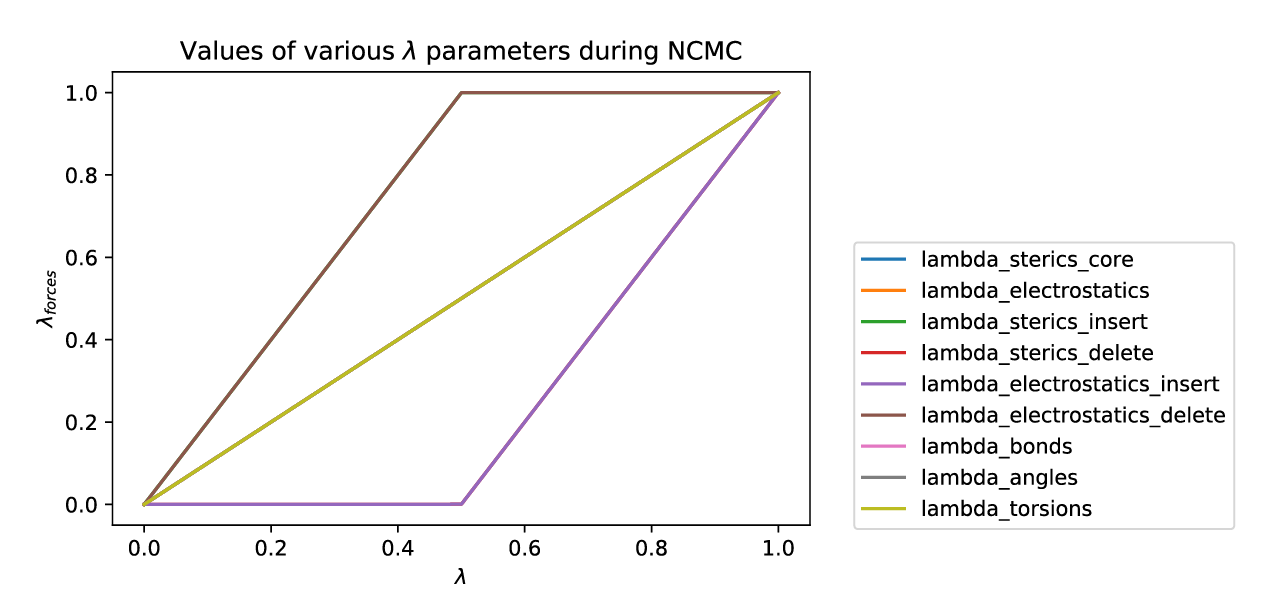
\includegraphics[width=0.8\textwidth]{lambda_traj_plotvec2-fixed.png}
    \caption{Nonbonded interpolation scheme, with the schedule of each individual force's $\lambda$ parameter plotted against the global $\lambda$. Note that sterics are always eliminated after electrostatics, and are always added before electrostatics. This provides protection against unshielded charges.}
    \label{fig:nb_interpolation}
\end{figure}
%
\subsubsection{Softcore sterics}
%
In order to provide greater simulation stability, I also utilize softcore sterics~\cite{Hornak2004}.
%
In this form, the sterics potential becomes:
\begin{eqnarray}
    U(r; \lambda_\mathrm{sterics}) &=& 4\epsilon\left[ \left(\frac{\sigma}{r}\right)^{12} - \left(\frac{\sigma}{r}\right)^6\right] \\
    \lambda_{\alpha} &=& \mathrm{dummy}_A (1-\lambda_\mathrm{sterics}) + \mathrm{dummy}_B (\lambda_{sterics}) \\
    \epsilon &=& (1 - \lambda_\mathrm{sterics}) \epsilon_A + \lambda_\mathrm{sterics} \epsilon_B \\
    \sigma &=& (1 - \lambda_\mathrm{sterics}) \sigma_A + \lambda_\mathrm{sterics} \sigma_B \\
    r_\mathrm{eff} &=& \sigma * \left[\alpha \lambda_\mathrm{sterics} (1 - \lambda_\mathrm{sterics}) + \left(\frac{r}{\sigma}\right)^6\right]^{1/6}
\end{eqnarray}
%
\noindent where $\mathrm{dummy}_A$ and $\mathrm{dummy}_B$ are parameters that determine whether the atom in question is a dummy atom at the initial endpoint or the final endpoint.
%
Though I did not explore this, the formulation includes an additional adjustable softcore parameter, $\alpha$. 
%
\subsubsection{Challenges with existing code bases}
%
The treatment of electrostatics controlled by a global parameter can be difficult, as particle mesh ewald~\cite{Darden1993} has a nontrivial efficient implementation. 
%
In this work, I leverage the ability of OpenMM~\cite{Eastman2017} to linearly interpolate charges while still calculating the full PME energy.
%
Without this, I was forced to implement only the direct space of the electrostatics term.
%
However, this resulted in the overlap between the hybrid system at the endpoints and the endpoint systems themselves being very poor, especially for charged ligands.
%
Therefore, it is advantageous to ensure that the full PME can be represented in the intermediate states.
%
\section{A note on ring closure}
%
One of the original motivations for pursuing the reversible jump algorithm was the ability to add complex ring systems, a task generally considered quite difficult for relative free energy calculations~\cite{Liu2015}.
%
However, as discussed in chapter 4, ring closure can be rather difficult, as the sequential importance sampling algorithm gradually produces weights that are increasingly poor.
%
While resampling in the geometry proposal appears attractive, it is very expensive; the need to compute many replicas of energy terms would require a highly optimized code for that purpose, and furthermore may suffer from numerical issues~\cite{Murray2016}
%
However, an appealing alternative would consist of simply softening the bonds and angles in the initial state of the hybrid system.
%
This would allow poorer proposals from the dimension matching system, instead cleaning up the poor geometries with annealing (which has the advantage of having tunable hyperparameters and running on the GPU).
%
Before running the entire solvent system, it is useful to examine how the softening of bonds and angles might affect the contribution of the initial jump to the hybrid system, known in the code as logP\_to\_hybrid.
%
In Figure~\ref{fig:bondsoftening}, one can see that the softer bond parameters significantly reduced the variance of the contribution of the jump to the hybrid system.
%
\begin{figure}
    \centering
    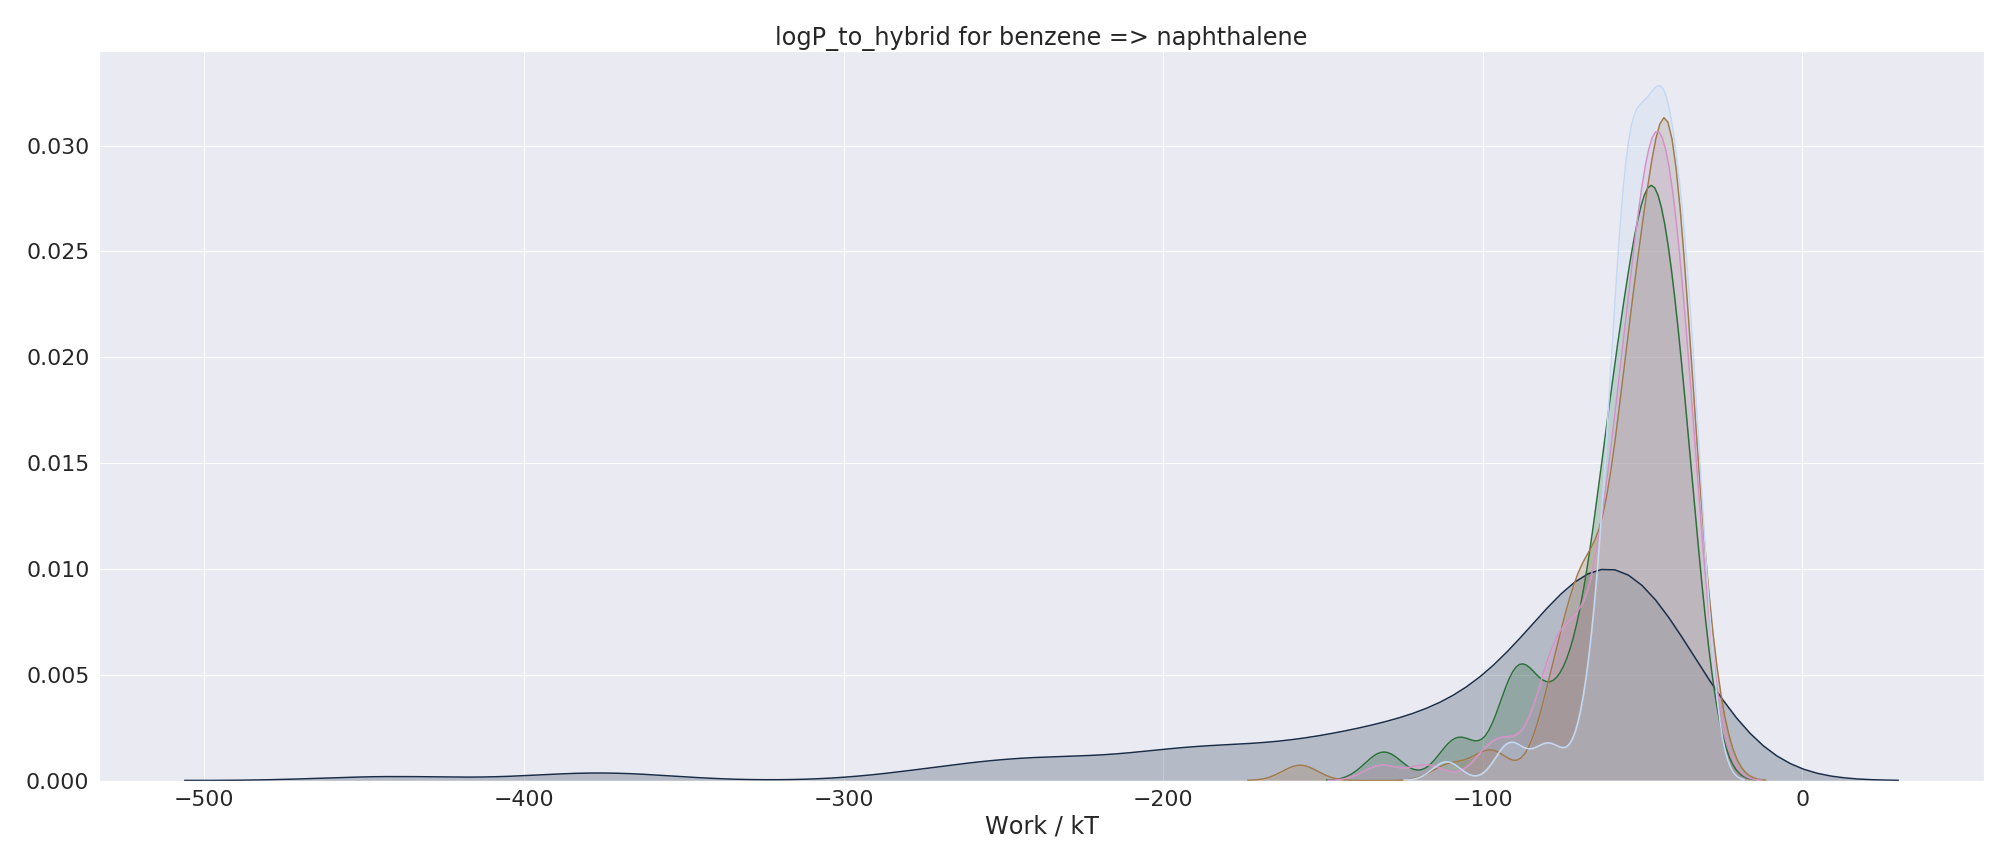
\includegraphics[width=\textwidth]{logP_tohybrid_changebond.png}
    \caption{The distributions of the logP\_to\_hybrid contribution under different initial bond softening parameters. The initial (darkest and broadest) distribution is with no softening; moving to lighter colors, we see the distribution narrow considerably as the initial force constants for bonds connecting unique atoms is scaled by 0.1, 0.01, 0.001, and 0.0001}
    \label{fig:bondsoftening}
\end{figure}
%
In addition to bonds, angles are also represented as harmonic terms, and so it behooves one to examine the effect of softening angles as well, under the same schedule. This time, we will hold the bond softening constant at 1.0 (no softening), and examine the effect of softening the angles in \ref{fig:anglesoftening}
%
\begin{figure}
    \centering
    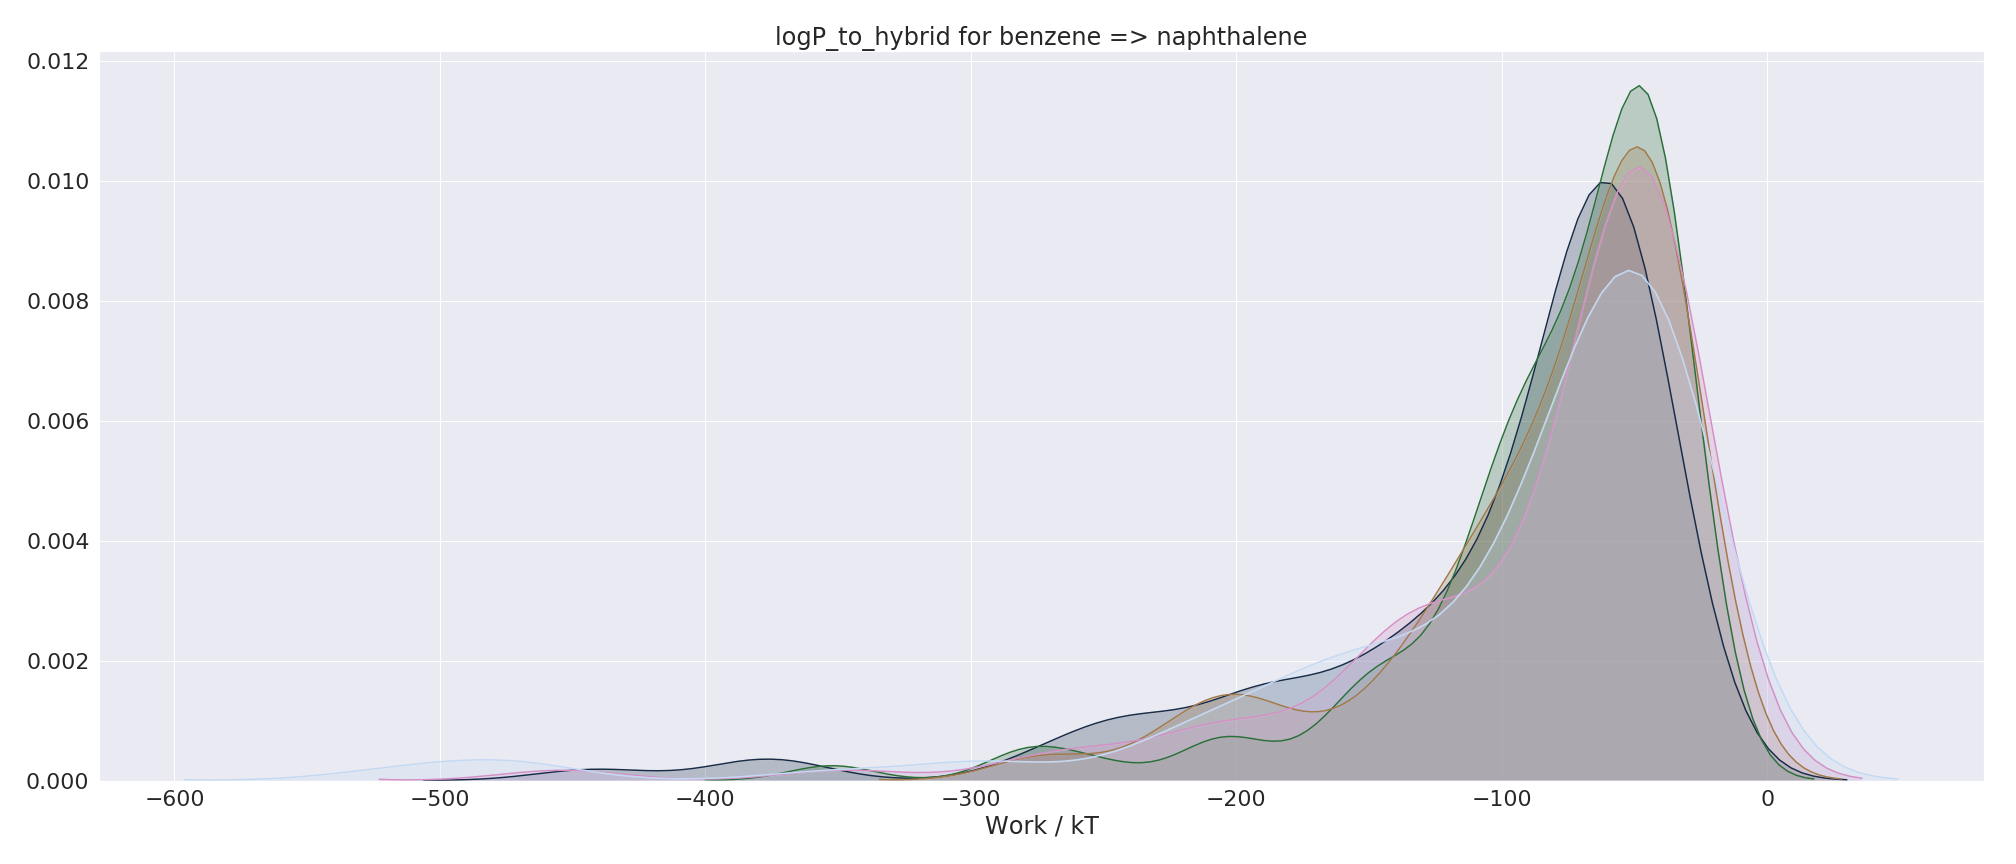
\includegraphics[width=\textwidth]{logP_tohybrid_changeangle.png}
    \caption{The distributions of the logP\_to\_hybrid contribution under different initial angle softening parameters. The initial (darkest and broadest) distribution is with no softening; moving to lighter colors, we do not see the same profound effect as the initial force constants for angles connecting unique atoms is scaled by 0.1, 0.01, 0.001, and 0.0001}
    \label{fig:anglesoftening}
\end{figure}
%
Interestingly, the angle terms do not seem to have the same profound effect as the bond terms.
%
An obvious explanation for this is that the force constants for the angles are considerably smaller, so it may require less softening.
%
In Figure~\ref{fig:softenboth}, I show the same softening schedule for both parameters.
%
\begin{figure}
    \centering
    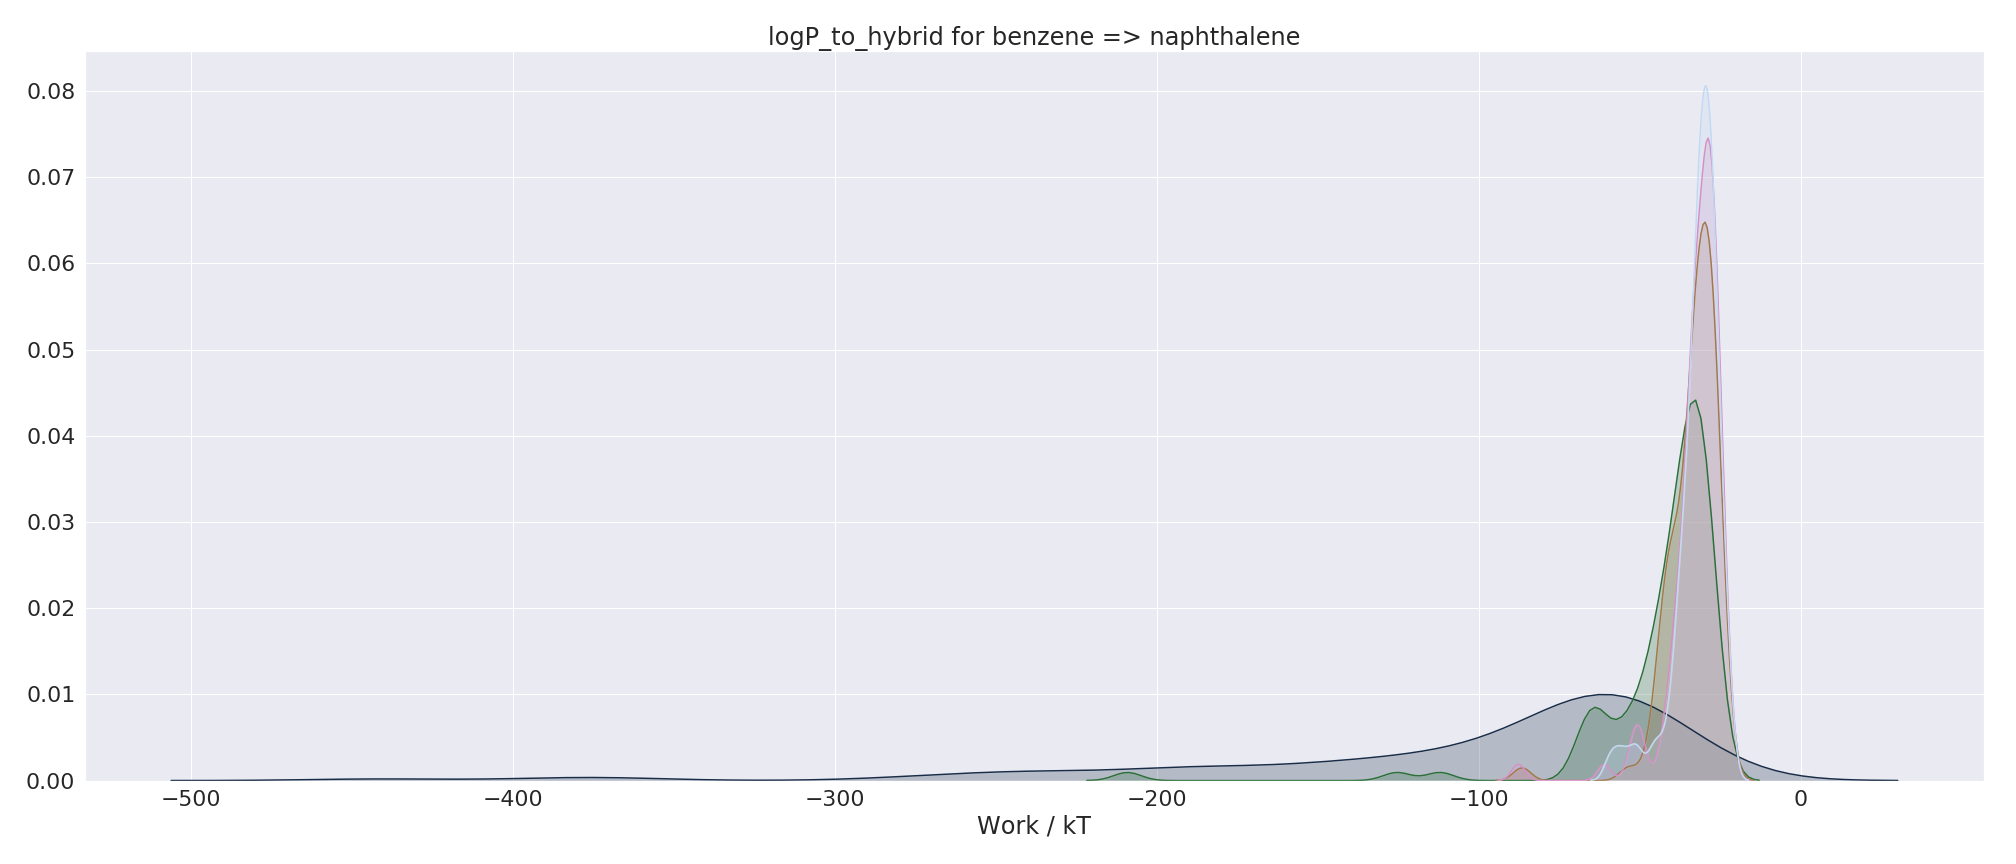
\includegraphics[width=\textwidth]{logP_tohybrid_changeboth.png}
    \caption{The distributions of the logP\_to\_hybrid contribution under different initial angle and bond softening parameters. The initial (darkest and broadest) distribution is with no softening; moving to lighter colors, we see that the distribution grows considerably narrower as both the angle and bond terms are softened to the same degree according to the schedule 0.1, 0.01, 0.001, 0.0001.}
    \label{fig:softenboth}
\end{figure}
%
Taking a closer look at the effect on the standard deviation of logP\_to\_hybrid, Figure~\ref{fig:angle_bond_softening} shows the effect of the different softening parameters on the standard deviation of the logP\_to\_hybrid component. Notably, the angles need not be softened as much as the bonds to reduce the variance of this component. The standard deviation of the standard deviations, obtained by bootstrapping, can be found in Figure~\ref{fig:stdstd}
%
\begin{figure}
    \centering
    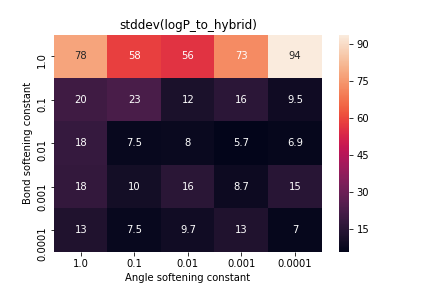
\includegraphics[width=0.8\textwidth]{std_nostd_to_hybrid.png}
    \caption{The standard deviation of the logP\_to\_hybrid component under different combinations of bond and angle softening constants. 
    It is noteworthy that the angles need not be softened nearly as much as the bonds.
    All quantities are in effective units of $k_B T$.
    }
    \label{fig:angle_bond_softening}
\end{figure}
%
\begin{figure}
    \centering
    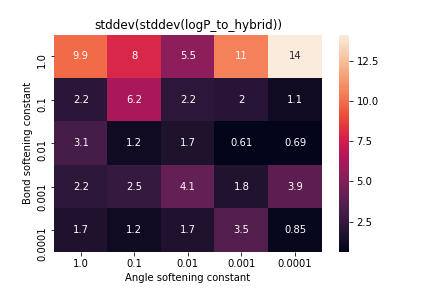
\includegraphics[width=0.8\textwidth]{stddev_lp.png}
    \caption{The standard deviations of the standard deviations of logP\_to\_hybrid under different combinations of bond and angle softening terms.
    All quantities are in effective units of $k_B T$.
    }
    \label{fig:stdstd}
\end{figure}
%
Although we can greatly diminish the variance of this quantity by simply softening the bonds, it is important to keep in mind that the ultimate objective is not to minimize the variance of the jump to the hybrid system, but rather to minimize the variance of the ultimate acceptance probability.
%
It is not difficult to imagine how excessive softening could negatively affect the overall acceptance probability, especially if the dimension matching distribution does not match the softened distribution.
%%
%
\section{Tuning NCMC Protocol length}
%
The simplest hyperparameter to tune in NCMC is the length of the switching protocol. The longer this protocol is, the more favorable the work values.
%
At the same time, the longer protocols require a greater amount of wall clock time.
%
At a certain point, the additional wall clock time consumed by the NCMC simulation is not worth the diminishing benefit in terms of work (which contributes directly to the acceptance probability).
%
Certain transformations may require a longer protocol than others; in this work, I use the same protocol length throughout a calculation.
%
%
\subsection{Limitations of tuning only length}
%
However, tuning the length alone, while straightforward, has limitations.
%
For instance, with a naive protocol linearly switching $\lambda$, it may be necessary to extend the protocol to many steps to ensure reasonable acceptance probabilities.
%
This approach does not give us the opportunity to more freely alter the schedule of the control parameters and potentially gain efficiency.
%
\subsection{Tuning Annealing Schedule}
%
However, with a protocol that may be nonlinear with the control parameter $\lambda$, we may afford ourselves an efficient protocol with many fewer steps.
%
The practical upshot of this is that a shorter protocol can achieve reasonable performance, provided the protocol is reasonable.
%
Unfortunately, as described previously, the thermodynamic length can be relatively difficult to calculate, and will vary depending 
%
\subsubsection{Theory}
%
%
In order to perform the experiment above, I first computed the thermodynamic metric tensor along the one dimensional path.
%
Then, I altered the schedule of control parameters to change $\lambda$ more rapidly when the metric tensor was small (indicating that neighboring distributions are similar) and more slowly when it is large (indicating that neighboring distributions may be quite far apart).
%
Although this sounds like a reasonable task, it is simplified in the case of the harmonic oscillator, where the metric tensor is available analytically.
%
Unfortunately, as is typically the case, the metric tensor is not available analytically for any molecular simulation of interest.
%
Thus, it must be estimated from sampling data, as described in \cite{Minh2011}.
%
This can be a rather expensive process, and may not be worth the added computation time.
%
\subsection{Limitations to tuning annealing schedule}
%
Despite the pleasant straightforwardness of using the metric tensor to define nonequilibrium switching protocols, there is another pitfall besides the computation cost: different pairs of ligands will have different metric tensors for their transformations, as well the same pair of ligands in different environments.
%
This means that it is not straightforward to transfer the values learned from one calculation into another.
%
Coupled with the computational cost, this may make the approach of using the thermodynamic metric tensor infeasible.
%
However, there may be alternate schemes that allow some degree of transfer learning.
%
\subsubsection{Simple solutions}
%
The simplest solution would be to perform a calculation with a number of different ligands in a common environment (such as explicit water) and trying to estimate a metric tensor for each of those transformations.
%
Then, one could potentially utilize a summary statistic of this collection of metric tensors in the hopes that on average, it will perform better than a naive protocol.
%
These approaches need to be explored in greater detail with a large number of different conditions
%
\subsubsection{General Solutions using Machine Learning}
%
In the future, one promising path forward is to use advances in machine learning to predict favorable alchemical paths.
%
In this paradigm, one might take many calculations in different environments, and learn a function $f_{\theta}(\mathcal{M}_1, \mathcal{M}_2)$ with optimizable parameters $\theta$ that maps a pair of molecules $\mathcal{M}_1$ and $\mathcal{M}_2$ to a reasonable schedule of control parameters.
%
Although appealing, it remains to be discovered how such a scheme would account for the myriad environments in which molecules find themselves in the course of a drug discovery program.
%
%
\subsection{Relationship to Geometry Tuning}
%
As mentioned earlier, there exists to some extent a tradeoff between the effort engaged in dimension matching and the effort spent in nonequilibrium switching.
%
More precisely, the more similar the hybrid system at the endpoint is to the non-modified system at the corresponding endpoints, the more straightforward the task of the dimension matching algorithm.
%
However, completely annihilating the valence interactions of newly-added atoms is also potentially dangerous.
%
Atoms that are not anchored to the molecule can easily drift far away, creating additional work as the bonds and angles are scaled on.
%
On the other hand, the dimension matching algorithm can essentially ignore the nonbonded interactions with surrounding atoms, as these are always decoupled at the beginning of the nonequilibrium switching protocol.
%
One question that remains is whether it is worthwhile to include the nonbonded interactions for the sake of maintaining favorable intramolecular nonbonded interactions.
%
%In Figure~\ref{fig:use_nonbonded}, we explore this tradeoff for a simple system of alkanes in vacuum, where %there are no other nonbonded interactions.
%
%\begin{figure}
%    \centering
%    \includegraphics{}
%    \caption{Average acceptance probability across all transitions for different lengths of NCMC with %nonbonded terms enabled in the dimension matching step (blue) and disabled (red).}
%    \label{fig:use_nonbonded}
%\end{figure}
%
\subsubsection{Possibility of resolving poor valence terms}
%
Although initially it seems that softening bonds is deleterious to the acceptance probability, the use of the dimension matching scheme without resampling means that small deviations from the target distribution can easily compound for large proposals.
%
As a result, it seems prudent to offer the choice of softening bonds, angles, and torsions between newly introduced atoms.
%
\nowidow[5]